\chapter{A Tale of Four Streams}

\section{Types of data streams}

Data streams come in many forms and sizes. They can be classified into four main 
categories for the sake of this course:

\begin{itemize}
    \item Myriads of tiny flows that you can collect, for example, coming from
    from physical or software sensors

    \item Continuos massive flows that you cannot stop, for example, from 
    telecomunications and utilities monitoring
    
    \item Continuous numerous flows that can turn into a torrent, like physical or cyber
    alarms

    \item Myriads of flows of any size and speed forming an inmense delta, like physical or
    software actuators
\end{itemize}

\section{Time models}

There are 3 main type of time models for streaming data analytics:

\begin{itemize}
    \item Stream-only time model
    \item Absolute time model
    \item Interval-based time model
\end{itemize}

\subsection{Stream-only time model}

In this model, time is defined by the order of the events in the stream. This model
is used when we only care about the order of the events, and not about the time that
they happened.\\

Therefore, in this model there is no notion of time, so this limits the type of queries
that we can do. This reduces the expresiveness of the model, but it also reduces the
latency of the system.

\subsection{Absolute time model}

In this model, time is defined by the time that the events happened. This model is 
useful when we need to know the exact time that the events happened, not only the order
in which they happened.\\

Therefore, in this model we can do more complex queries, like time-based queries or
window-based queries. This increases the expressiveness of the model, but it also
increases the latency of the system.

\subsection{Interval-based time model}

In this model, time is defined by intervals. This model is useful when we need to know
the time that the events happened, but we also need to group the events in intervals.\\

Therefore, in this model we can do more complex queries, not only time-based queries,
but also group the events in specific intervals. This increases the expressiveness of
the model, but it also increases the latency of the system.

\subsection{Trade-off: latency vs expressiveness}

There is a trade-off between latency and expressiveness. Let us see the following 
graph:

\begin{figure}[H]
    \centering
    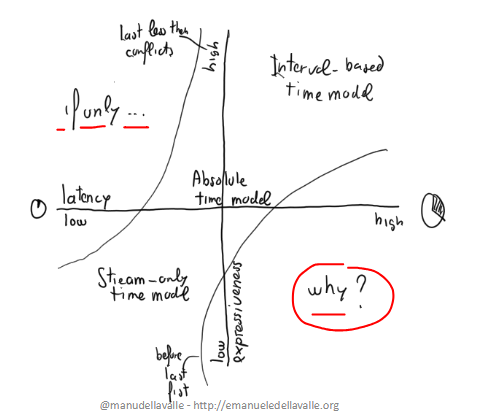
\includegraphics[width=0.7\textwidth]{figures/image_express_vs_lat.png}
    \caption{Trade-off between latency and expressiveness}
    \label{fig:trade-off-lat-expr}
\end{figure}

\section{Architectures for stream processing}

There are four main architectures for stream processing:

\begin{itemize}
    \item Event-based systems
    \item Data Stream Management Systems
    \item Complex Event Processing
    \item Event-driven architecture
\end{itemize}


\subsection{Event Based Systems (EBS)}

An Event-Based System is a software architecture paradigm in which data flows
and operations are driven by events rather than following a pre-defined control
flow. In other words, in an EBS, actions are executed in response to specific events
that occur, rather than as a part of a predetermined logical sequence.\\

Two main concepts:

\begin{itemize}
    \item Event: an immutable and append-only stream of "business facts" that are
    generated by sensors, applications, or users.
    \item Decoupling: means decentralizing the freedom to act, adapt and change
\end{itemize}

There are two main types of event-based systems:

\begin{itemize}
    \item Content-based systems
    \item Topic-based systems
\end{itemize}

\subsubsection{Content-based systems}

Content-based systems filter and route messages based on the actual content within
the messages. In this model, subscribers specify their interest through content attributes,
and the system delivers only messages that match these attributes.\\

This type of systems are mainly used as an academic effort, as they are hard to implement
in practice.

\subsubsection{Topic-based systems}

Topic-based systems organize messages by predefined topics. In this model, publishers
send messages to a specific topic, and subscribers receive all messages sent to the topic
they have subscribed to.\\

This type of systems are the most common in practice, and they are widely available for
industrial applications. Some examples are Apache Kafka, MQTT, among others.

\subsubsection{Kafka: "the" event-based system}

Apache Kafka is a distributed event streaming platform that is capable of handling trillions
of events a day. It is used by thousands of companies to build real-time streaming data pipelines
and applications.\\

In this system, topics are partitioned into kafka brokers. Producers share messages over
the partitions on a certain topic via hash partitioning or round-robin partitioning. 
Different consumers can read messages from the same topic, and partitions guarantee
parallel reads.\\

\subsection{Data Stream Management Systems (DSMS)}

Data Stream Management Systems (DSMS) are systems that are designed to handle
continuous massive flows of unstoppable data. They are used to process and analyze
data streams in real-time.\\

Data streams are sequences (sometimes unbounded) of time-varying data elements. They 
represent an almost continuos flow of information, with the most recent information
being more relevant, as it describes the current state of a dynamic system.\\

The nature of streams require a paradigmatic change, from persistent data (one-time 
semantics) to transient data (continuous semantics). 

\subsubsection{DSMS semantics}

This syem uses continuos queries registered over streams that are observed through
a window, like the following picture:

\begin{figure}[H]
    \centering
    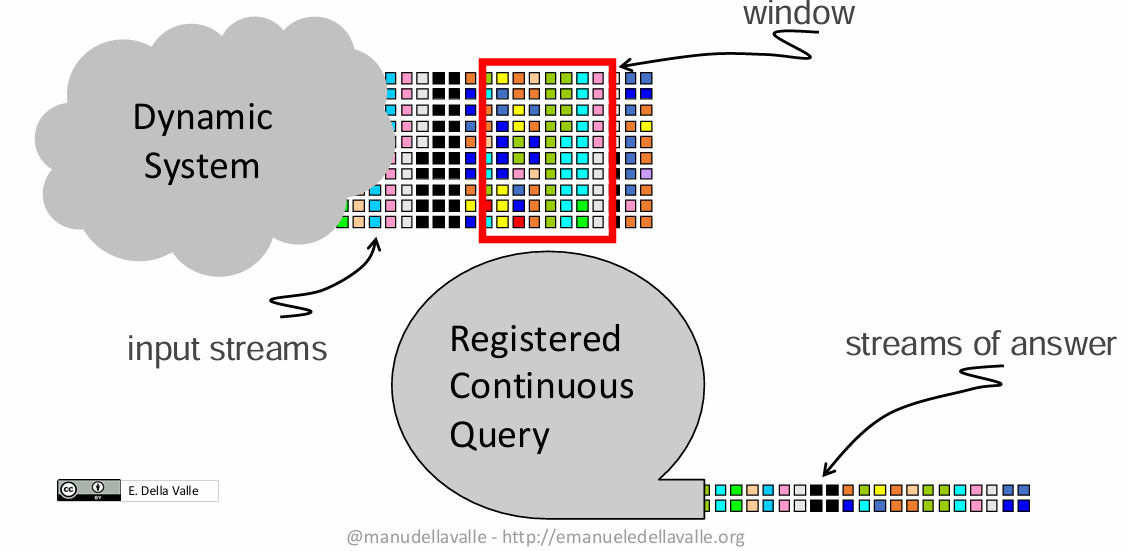
\includegraphics[width=0.7\textwidth]{figures/image_DSMS.png}
    \caption{DSMS semantics}
    \label{fig:1}
\end{figure}

We can do different operations over the data stream. For example, we can do incremental
operations, like:

\begin{itemize}
    \item[$\rightarrow$] Filtering (more generally, mapping)
    \item[$\rightarrow$] Grouping
    \item[$\rightarrow$] Count, sum, min, max, means
    \item[$\rightarrow$] Variance and standard deviation
\end{itemize}

Specially, for variance calculation, we can use the Welford's algorithm, which is an
online algorithm for calculating the variance of a sample. It is more numerically stable
than the standard formula for variance, and it is also more efficient. The algorithm
is as follows:

\begin{algorithm}[H]
    \caption{Welford's algorithm}
    \begin{algorithmic}[1]
        \State $n \gets 0$
        \State $\mu \gets 0$
        \State $M2 \gets 0$
        \State
        \Procedure{update}{$x$}
            \State $n \gets n + 1$
            \State $\delta \gets x - \mu$
            \State $\mu \gets \mu + \frac{\delta}{n}$
            \State $\delta_2 \gets x - \mu$
            \State $M2 \gets M2 + \delta \cdot \delta_2$
        \EndProcedure
    \end{algorithmic}
\end{algorithm}

However, there are some operations that we are not able to exactly 
calculate with continuos semantics, like the median, mode, top-k, distinct count, etc.
For some of these operations, we can use approximations.

\subsubsection{Window types}

There are three main types of windows in DSMS:

\begin{itemize}
    \item Sliding window: a window that slides over the stream
    \item Tumbling window: a window that is fixed in time
    \item Session window: a window that groups events that are close in time
\end{itemize}

Note that we are not specifying the time model. This is because DSMS can work with
any time model, as long as it is specified in the query. For example, if we are working
with the stream-only time model, we define physical windows. E.g.: for a tumbling window,
every 10 events; for a sliding window, consider the last 10 events every 5 events; Note
that session windows cannot be specified.\\

If we consider an absolute time model, we define logical windows. E.g.: for a tumbling
window, every 10 seconds; for a sliding window, consider the last 10 seconds every 5 seconds;
for a session window, every 10 seconds of inactivity.\\

An example of a windowed aggregation query in DSMS is the following:\\

\begin{lstlisting}[language=SQL]
SELECT STREAM
    HOP_END(rowtime, INTERVAL '1' HOUR, INTERVAL '3' HOUR),
    COUNT(*),
    SUM(units)
FROM Orders
GROUP BY 
    HOP(rowtime, INTERVAL '1' HOUR, INTERVAL '3' HOUR);
\end{lstlisting}

\subsubsection{Streaming joins}

A streaming join is an operation that combines two or more streams based on a common
key or specific attribute.\\

In traditional databases, combining rows from different tables is a basic operation, but 
in stream processing is hard because the data is not static but in constant motion.\\

Streams are data that flows over time. Therefore, joins consider the temporal sycronization
of the data via time windows to limit the join to events that occur within a certain time
interval.\\

An example:

\begin{lstlisting}[language=SQL]
SELECT STREAM o.rowtime o.productId, o.orderId,
            s.rowtime AS shipTime
FROM Orders AS o JOIN Shipments AS s 
    ON o.orderId = s.orderId AND
        s.rowtime BETWEEN 
            o.rowtime AND 
            o.rowtime + INTERVAL '1' HOUR;
\end{lstlisting}


\subsection{Complex Event Processing (CEP)}

Complex Event Processing (CEP) is a method of tracking and analyzing streams of information
from different sources to identify patterns and relationships. It is used to process and analyze
data streams in real-time.\\

CEPs add the ability to deploy rules that describe how composite events can be generated from
primitive ones. Typical CEP rules search for sequences of events that match a pattern, for
example: \texttt{Raise C if A $\rightarrow$ B}. Time is a key factor in CEP, as it is used to
determine the order of events and the time window in which the events must occur.\\

\subsubsection{CEP semantics}

Complex Event Processing (CEP) uses subsets of Allen's interval algebra to define the temporal
relationships between events. The main operators are:

\begin{figure}[H]
    \centering
    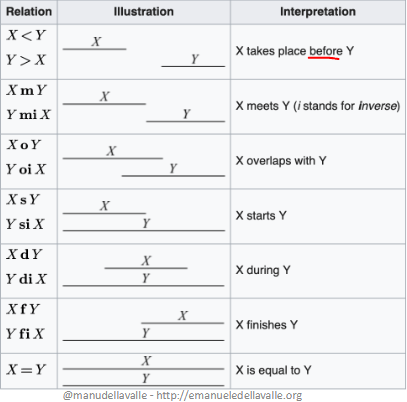
\includegraphics[width=0.5\textwidth]{figures/image_Allen_interv_alg.png}
    \caption{Allen's interval algebra}
    \label{fig:interval_alg}
\end{figure}

\subsubsection{Event Processing Language (EPL)}

Event Processing Language (EPL) is a language that is used to 
define rules in CEP. It has the capability to describe complex
event patterns and relationships, to create queries that monitor
real-time data streams.\\

It is supported by many CEP engines. The main engine we are going to use 
in this course is Esper, although there are others like Oracle CEP.\\

An example of a query in EPL is the following:\\

\begin{lstlisting}[language=SQL]
insert into alertIBM
select *
from pattern [
    every (
        StockTick(name="IBM", price > 100)
        ->
        (StockTick(name="IBM", price < 100)
            where timer:within(60 seconds))
    )
];
\end{lstlisting}

This query alerts on each IBM stock tick with a price gretaer than 100,
followed by a tick with a price less than 100 within 60 seconds.\\

\subsection{Event-driven Architecture}

Event-driven architecture is a software architecture paradigm promoting the production,
detection, consumption of, and reaction to events. An event can be defined as a significant
change in state.\\

In this paradigm, the system only worries about writing the events to the event log, and
the rest of the system can react to these events. This allows for a more decoupled system,
where each consumer can read react to the events asyncronously.\\

\begin{figure}[H]
    \centering
    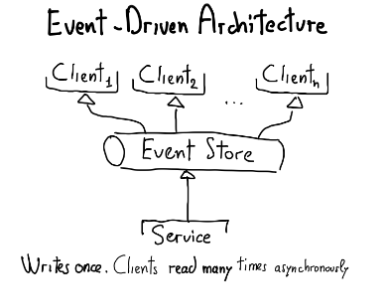
\includegraphics[width=0.5\textwidth]{figures/image_EDA.png}
    \caption{Event-driven architecture}
    \label{fig:event_driven_arch}
\end{figure}

EDAs have two main functionalities:

\begin{itemize}
    \item Notifications, which is just a stream of observations
    \item Data replication, which is a stream of changes
\end{itemize}
